\chapter{Design}
\paragraph{}
In this chapter, we begin by presenting the main structure of the app, and then we further detail the different objects and libraries that have been implemented throughout the project.

\paragraph{}
The app itself uses a side drawer component to navigate between the main parts, such as the home screen, CISC, PoP, and settings. Each of these drawers then splits in multiple tabs if needed in order to separate sub-sections of each component. In each tab, only the functionalities available to this sub-section of the component can be found. The following list shows the main structure of the app, such that each main point is a drawer and each sub-point is a tab.

\begin{itemize}
\item Home \linebreak The home screen displays the conodes of the user. One can add and remove conodes, fetch their statuses and display them as a QR code.

\item PoP
\begin{itemize}
\item PoP \linebreak Used to display data shared between attendees and organizers, it shows the list of all the fetched final statements and generated PoP tokens.

\item Org \linebreak Contains all the functionalities needed by the organizers of a PoP party.
\end{itemize}

\item CISC // TODO: INSERT

\item Settings
\begin{itemize}
\item User \linebreak The settings of the user include key pair generation and displaying, one can also completeley reset the data linked to the user of the app.

\item CISC // TODO: INSERT

\item PoP \linebreak In this tab one can reset the global PoP data and the data linked to the organizer.
\end{itemize}
\end{itemize}

\paragraph{}
In order to easily represent the information, manage the data, and use the corresponding functionalities for all of these components, we chose to create multiple JS classes that are true singletons (as far as JS allows). Singletons permitted us to always work on the exact same object independently from the location we require for the class; since we had to store data locally, we had to load the saved states into memory for each of these classes. Thanks to the singleton design pattern, this loading must only be executed once, either at the start-up of the app or the first time the class is required, and all subsequent calls use this pre-loaded object. On the other hand, since we work with singletons, we were not able to create relationships between them; for example, the class that represents the organiser of a PoP party does not extend the main PoP class (each subclass instance would recreate their own parent class instance). The classes that have been implemented are listed below.

\begin{itemize}
\item User.js \linebreak Contains all the data and logic that is global and belongs to the user of the app. At this state the user class manages the key pair and the roster displayed in the home screen.

\item Cisc.js // TODO: INSERT

\item PoP.js \linebreak Contains everything that is common to organizers and attendees, it manages the list of final statements and PoP tokens belonging to the user.
\begin{itemize}
\item Att.js \linebreak This class is only a skeleton for now and not used at all. It is a placeholder for future implementations that are specific to the attendees of a PoP party.

\item Org.js \linebreak Represents the organizer of a PoP party. This class manages the current linked conode, PoP configuration, registered attendees and ID of the PoP description.
\end{itemize}
\end{itemize}

\paragraph{}
In addition to these objects, we wrote some libraries so that we can easily manipulate any kind of data, be it local or exchanged with conodes. The main libraries are presented as follows.

\begin{itemize}
\item Convert.js \linebreak Library for converting data types but also to parse all kind of stored data.

\item Crypto.js \linebreak Everything related to cryptography which includes but is not limited to key pair generation, message signing and verification or EC points aggregation.

\item Helper.js \linebreak All kind of helper functions that may be needed in several different places but do not belong to any other library.

\item Net.js \linebreak Contains all the methods related to communication over the internet, may it be over websockets or HTTP requests.

\item protobuf/ \linebreak Creation, encoding, decoding and more using protocol buffers to efficiently use the same object structure as the CISC and PoP implementations in Go\footnote{\url{https://golang.org}} from the DeDiS lab.
\end{itemize}

\paragraph{}
The classes and libraries in combination provide any required logic to execute the CISC and PoP apps locally but also to perform any communication needed with the conodes. We chose to implement these in such a way that it not only can be taken out as a whole and used as a library with as few tweaks and changes as possible for any other JS project related to the Cothority framework, but also so that it is easily extensible for other Cothority apps that will one day be implemented. We decided to call this aggregation of libraries "DeDjS".
Throughout the entire project, any data like keys, IDs, or EC points were handled as unsigned byte arrays (Uint8Array in JS) but shown to the user in the base64\footnote{\url{https://en.wikipedia.org/wiki/Base64}} format (unless explicitly stated otherwise). This choice combines an easy way of handling the data and an easy way for the user to read the data on the screen. Moreover, since JS is an un-typed language, we decided to implement DeDjS so that it is as type safe as possible. This choice of implementation was made to prevent simple errors and return meaningful exception messages when a required type is incorrect.

\paragraph{}
Much of the logic in DeDjS requires writing and reading data to and from the disk or sending messages over the internet in order to use the functionalities of Cothority. These tasks are slow, generate delays, and even have a relatively high probability of failing. One of the challenges was to find a way to execute all of these tasks in an asynchronous way so as to not block the main thread of the app and handle exceptions in a simple and clean manner. The solution to this problem was that, since ECMAScript\footnote{\url{https://en.wikipedia.org/wiki/ECMAScript}} 2015, it is possible to use promises\footnote{\url{https://en.wikipedia.org/wiki/Futures_and_promises}} in JS. Thus, we decided to implement DeDjS so that it uses promises anytime an asynchronous task is needed. In this way, the main thread of the app is never blocked, and the exceptions can easily be handled by the simple syntax provided by JS.

\begin{figure}[h]
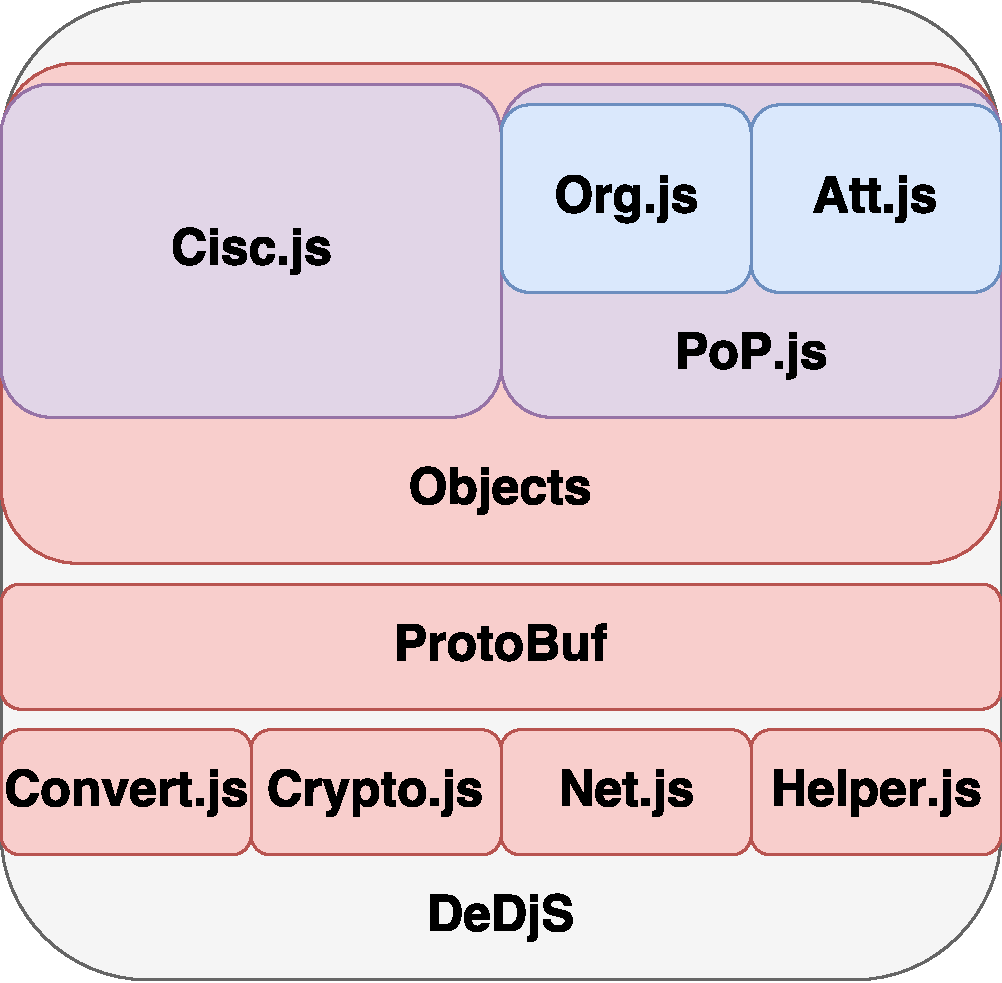
\includegraphics[scale=.5]{graphic/dedjs.pdf}
\centering
\caption{DeDjS Library Structure}
\end{figure}
